% ====================================================================
% AAAI 2027 Main-Track Submission
% Hierarchical Multi-Agent Wildfire Suppression
% ====================================================================
\documentclass[letterpaper]{article}
% [submission] mode: anonymized review format; the style itself loads the required
% fonts (newtxtext/helvet/courier) and owns page geometry — do not load times or
% set \pdfpagewidth manually (forbidden by aaai2027.sty).
\usepackage[submission]{aaai2027}
\usepackage[hyphens]{url}
\usepackage{graphicx}
\urlstyle{rm}
\def\UrlFont{\rm}
\usepackage{natbib}
\frenchspacing

\usepackage{amsmath}
\usepackage{amssymb}
\usepackage{booktabs}
\usepackage{multirow}
\usepackage{algorithm}
\usepackage{algorithmic}
\usepackage{tikz}
\usetikzlibrary{shapes.geometric, arrows.meta, positioning}

\pdfinfo{
/Title (Hierarchical Strategic Coordination for Infrastructure-Aware Wildfire Suppression under Realistic Physics)
/Author (Anonymous)
/TemplateVersion (2027.1)
}

\setcounter{secnumdepth}{2}

\title{Hierarchical Strategic Coordination for \\ Infrastructure-Aware Wildfire Suppression \\ under Realistic Physics}
\author{Anonymous Authors}
\affiliations{Anonymous Affiliations}

\begin{document}
\maketitle

% ====================================================================
% ABSTRACT
% ====================================================================
\begin{abstract}
Coordinating multi-agent teams to defend critical infrastructure during wildfires is a spatial-temporal decision problem that couples strategic asset prioritization with local suppression. We contribute an \emph{infrastructure-aware wildfire-coordination benchmark} built on the validated Cell2Fire physics engine and two documented, GIS-derived landscapes---Saudi Arabian petroleum infrastructure and California Wildland-Urban Interface (WUI) zones---together with a rigorous, fully reproducible evaluation of decentralized, communication-based, hierarchical, and heuristic controllers under a uniform 5-seed $\times$ 15-episode protocol. Our study yields three findings. First, the benchmark is \emph{diagnostic}: policy classes reverse rank across regions---a learned communication policy (CommNet) is strongest on concentrated petroleum assets (Weighted Economic Loss $11.4$ vs.\ $27.0$ for no-operation), whereas simple reactive coverage is strongest on scattered WUI assets---so no single method dominates. Second, we isolate a concrete failure mode: even with a matched objective and a $10\times$ larger training budget, \emph{communication-free} MAPPO fails to defend concentrated infrastructure, remaining at the no-operation loss level while operating, on average, $6.8$ cells from the nearest asset. Third, a behavior-cloned, KL-regularized hierarchical commander serves as an interpretable reference solution with compliance guaranteed by construction; we show through equivalence testing that it is \emph{comparable to but not statistically equivalent to} its expert teacher, and through a falsifiable generalization metric that its learned sector preferences do not transfer to rotated layouts or across regions. We release code, checkpoints, GIS pipeline, and a hashed reproducibility manifest.
\end{abstract}

% ====================================================================
% 1. INTRODUCTION
% ====================================================================
\section{Introduction}
\label{sec:intro}

Wildfire suppression demands coordinated allocation of limited suppression resources across a dynamically evolving hazard landscape. When critical infrastructure---petroleum refineries, pipeline junctions, residential structures---lies in the path of an advancing fire front, the coordination challenge intensifies: agents must \emph{strategically prioritize} which assets to defend rather than simply minimizing total burned area. This infrastructure-defense framing distinguishes wildfire suppression from generic fire-containment problems and motivates the present work.

\paragraph{Problem: When does decentralized MARL fail?}
Standard decentralized MARL algorithms such as MAPPO \citep{yu2022mappo} and QMIX \citep{rashid2018qmix} equip agents with local egocentric observations and learn decentralized policies via centralized training. A recurring concern is that, under partial observability, agents cluster near locally visible fire and fail to allocate effort toward distant high-value assets. Rather than assert this failure in general, we treat it as an empirical question and give it a fair test: we train each baseline for a $10\times$ larger budget on the \emph{same} infrastructure-weighted objective used for evaluation. The result is region-dependent (Section~\ref{sec:results}): on concentrated petroleum infrastructure, communication-free MAPPO indeed fails---its Weighted Economic Loss is indistinguishable from taking no action---while on scattered residential assets it partially succeeds, and a learned \emph{communication} baseline succeeds in both. The failure is thus specific, not universal, and the benchmark's value is precisely that it separates these cases.

\paragraph{A reference solution and the compliance gap.}
Hierarchical reinforcement learning (HRL) offers one structured remedy: a strategic commander that dispatches agents to priority sectors. A systems-level subtlety, however, is that if low-level agents do not reliably \emph{comply} with strategic directives, the commander's decisions decouple from physical outcomes---we call this the \emph{compliance gap}. We adopt a design that closes this gap by construction: (1) a \textbf{strategic commander} assigns each agent to one of $M = 16$ spatial sectors every $T_{\text{macro}} = 10$ steps, and (2) a deterministic \textbf{target-seeking policy} routes agents to their assigned sectors, so compliance is guaranteed rather than learned. We present this hierarchy as an \emph{interpretable reference solution} rather than a performance-maximizing method: it matches its behavior-cloned expert teacher (though, as we show by equivalence testing, it is not statistically equivalent to it) and is a transparent point of comparison for the benchmark.

\paragraph{Contributions.} Our contributions are:
\begin{enumerate}
    \item An \textbf{infrastructure-aware wildfire-coordination benchmark} on the validated Cell2Fire physics engine and two documented, GIS-derived landscapes (Saudi petroleum and California WUI), with a released data pipeline and hashed manifests.
    \item A \textbf{diagnostic evaluation} of decentralized (MAPPO, QMIX), communication-based (CommNet), heuristic, and hierarchical controllers under a uniform protocol, showing that policy classes reverse rank across regions and pinpointing a concrete failure mode of communication-free MARL on concentrated assets---supported by training curves and behavioral analysis.
    \item A \textbf{hierarchical reference solution} with compliance guaranteed by construction, plus a \textbf{compliance-diagnostics} framework (adherence, dispatch latency, reassignment rate) that quantifies how strategic intent maps to physical behavior.
    \item A \textbf{rigorous statistical protocol}---5 seeds, bootstrap 95\% CIs, Welch's $t$-tests with reported degrees of freedom, TOST equivalence testing, and a falsifiable generalization metric---applied uniformly across all claims.
\end{enumerate}

% ====================================================================
% 2. RELATED WORK
% ====================================================================
\section{Related Work}
\label{sec:related}

\paragraph{Wildfire Simulation and GIS-Based Planning.}
Wildfire spread modeling has progressed from simple cellular automata to physics-based simulators. Cell2Fire \citep{pais2021cell2fire} implements the Canadian Forest Fire Behavior Prediction (FBP) system with heterogeneous fuel types, wind effects, and topographic slope corrections. Operational research approaches optimize firebreak placement using mixed-integer programming \citep{hu2009wildfire} but assume global state observability and static fire behavior, neither of which holds during active suppression. Our work uses Cell2Fire as a validated physics backend while framing suppression as a sequential decision problem under partial observability.

\paragraph{Reinforcement Learning for Wildfire and Disaster Response.}
Recent RL approaches to wildfire include UAV-based detection \citep{ghali2022, partheepan2023}, landscape-scale fuel-treatment planning \citep{altamimi2022wildfire}, and grid-based suppression agents on Cell2Fire \citep{shen2022firehose}. Most use simplified fire dynamics without validated physics, single-agent formulations, or toy grids that lack realistic infrastructure; the closest prior system, Firehose \citep{shen2022firehose}, is single-objective (burned-area) and single-agent. To our knowledge, no prior work targets \emph{multi-agent, infrastructure-weighted} suppression on a validated physics engine, which is the gap our benchmark addresses; we make no claim of algorithmic novelty in the hierarchical controller itself. Operations-research approaches remain the deployed state of the art for suppression \emph{planning}: they optimize firebreak or resource placement via mixed-integer programming \citep{hu2009wildfire} under global observability and quasi-static fire, and are complementary to---not competitors of---the sequential, partially observed, reactive-suppression setting we study. Disaster-response RL more broadly has explored resource allocation \citep{nguyen2019disaster} but rarely the spatial coordination of multi-agent infrastructure defense under physically grounded fire spread.

\paragraph{Cooperative MARL and Communication.}
Centralized Training with Decentralized Execution (CTDE) is the dominant paradigm for cooperative MARL. QMIX \citep{rashid2018qmix} factorizes joint value functions under monotonicity constraints; MAPPO \citep{yu2022mappo} applies PPO \citep{schulman2017} with centralized critics. CommNet \citep{sukhbaatar2016learning} and TarMAC \citep{das2019tarmac} add learned communication channels. A common assumption is that agents can learn implicit coordination from reward signals alone. We test this directly on our benchmark and find it holds only partially: communication-free MAPPO fails to defend concentrated infrastructure even with a fair budget, whereas adding a CommNet communication channel recovers strong performance---evidence that the operative bottleneck is inter-agent coordination rather than low-level skill.

\paragraph{Hierarchical Reinforcement Learning.}
The options framework \citep{sutton1999options} and feudal networks \citep{vezhnevets2017feudal} introduce temporal abstraction via subgoal hierarchies. HAM \citep{parr1998hams} and MAXQ \citep{dietterich2000maxq} decompose MDPs into subtask hierarchies. In multi-agent settings, RODE \citep{wang2021rode} uses role decomposition, while MAVEN \citep{mahajan2019maven} conditions on shared latent variables. Most prior HRL work uses \emph{learned} low-level policies that are jointly optimized with the high-level controller. A key distinction of our approach is that we \emph{deliberately decouple} the tactical layer into a deterministic target-seeking policy, which guarantees that strategic decisions control spatial allocation and enables direct compliance measurement.

\paragraph{Imitation Learning and RL Fine-Tuning.}
Combining imitation with RL is well-established: DAgger \citep{ross2011reduction} iteratively corrects distributional shift; behavioral cloning followed by RL fine-tuning has been applied to game playing \citep{silver2016mastering} and robotics \citep{rajeswaran2017learning}. KL-regularized policy optimization prevents catastrophic forgetting of imitation priors \citep{wu2019behavior}. We apply this paradigm to hierarchical wildfire coordination, using a domain-expert value-weighted heuristic as the BC teacher for the strategic commander.

% ====================================================================
% 3. PROBLEM FORMULATION
% ====================================================================
\section{Problem Formulation}
\label{sec:formulation}

We model wildfire suppression as a Decentralized Partially Observable Markov Decision Process (Dec-POMDP) extended with hierarchical temporal abstraction.

\paragraph{State.}
The global state $s = \langle S_{\text{fire}}, S_{\text{asset}}, S_{\text{agent}} \rangle$ consists of:
\begin{itemize}
    \item $S_{\text{fire}} \in \{0,1\}^{H \times W}$: binary active-fire grid evolved by Cell2Fire physics.
    \item $S_{\text{asset}} \in \mathbb{R}_{\geq 0}^{H \times W}$: infrastructure criticality map encoding economic asset values.
    \item $S_{\text{agent}} = \{(y_i, x_i)\}_{i=1}^N$: grid positions of $N$ suppression agents.
\end{itemize}

\paragraph{Observations.}
Each agent $i$ observes an egocentric $C \times C$ crop ($C = 9$) containing 8 channels: active fire, treated cells, fuel type, criticality, agent occupancy, normalized coordinates, fire fraction, and time fraction. Agents do \emph{not} observe the full grid.

\paragraph{Actions.}
Micro-actions $a_i^t \in \{$stay, up, down, left, right, treat$\}$ are executed at every environment step. Macro-actions $a_i^{\text{macro}} \in \{0, \dots, M{-}1\}$ assign agents to one of $M = 16$ spatial sectors (a $4{\times}4$ partition of the grid), selected every $T_{\text{macro}} = 10$ steps.

\paragraph{Reward.}
The macro-level reward for the strategic commander is:
\begin{equation}
\label{eq:reward}
R^{\text{macro}} = -\Delta \text{WEL} + \alpha \cdot \Delta \text{ISR}
\end{equation}
where $\text{WEL} = \sum_j v_j \cdot \mathbf{1}[\text{asset}_j \text{ burned}]$ is the Weighted Economic Loss, $\text{ISR} = |\{\text{surviving assets}\}| / |\{\text{total assets}\}|$ is the Infrastructure Survival Rate, and $\alpha = 20$ upweights survival. This reward directly incentivizes infrastructure defense over generic burned-area minimization.

% ====================================================================
% 4. METHODOLOGY
% ====================================================================
\section{Methodology}
\label{sec:method}

% --- Figure 1: Architecture Diagram Placeholder ---
% --- Figure 1: Architecture Diagram in TikZ ---
\begin{figure}[t]
    \centering
    \resizebox{\columnwidth}{!}{
    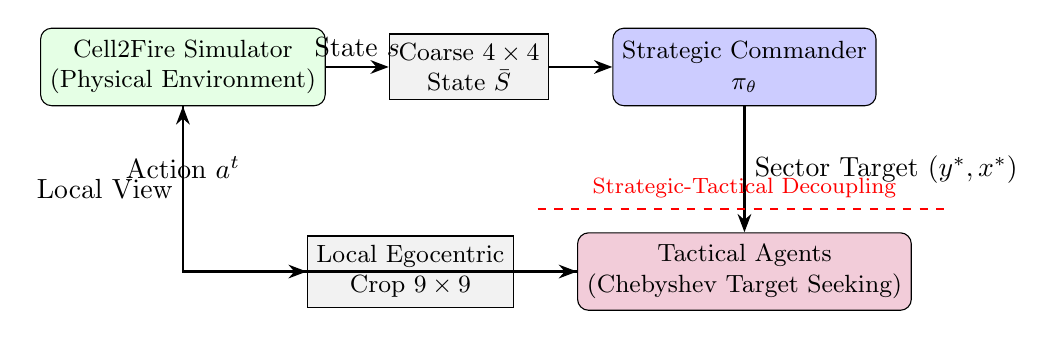
\begin{tikzpicture}[
        node distance=1.2cm and 0.8cm,
        block/.style={draw, fill=blue!10, rectangle, minimum height=2.8em, minimum width=6em, rounded corners, align=center, font=\small},
        input/.style={draw, fill=gray!10, rectangle, minimum height=2.2em, minimum width=5em, align=center, font=\small},
        env/.style={draw, fill=green!10, rectangle, minimum height=2.8em, minimum width=7em, rounded corners, align=center, font=\small},
        arrow/.style={-{Stealth[scale=1.0]}, thick}
    ]
        % Nodes
        \node (env) [env] {Cell2Fire Simulator\\(Physical Environment)};
        \node (coarse) [input, right=of env] {Coarse $4 \times 4$\\State $\bar{S}$};
        \node (commander) [block, fill=blue!20, right=of coarse] {Strategic Commander\\$\pi_\theta$};
        \node (tactical) [block, fill=purple!20, below=of commander, yshift=-0.4cm] {Tactical Agents\\(Chebyshev Target Seeking)};
        \node (local) [input, left=of tactical] {Local Egocentric\\Crop $9 \times 9$};
        
        % Paths
        \draw [arrow] (env) -- (coarse) node[midway, above] {State $s$};
        \draw [arrow] (coarse) -- (commander);
        \draw [arrow] (commander) -- (tactical) node[midway, right] {Sector Target $(y^*, x^*)$};
        \draw [arrow] (env) |- (local) node[pos=0.25, left] {Local View};
        \draw [arrow] (local) -- (tactical);
        \draw [arrow] (tactical) -| (env) node[pos=0.75, above] {Action $a^t$};
        
        % Decoupled boundary annotation
        \draw[dashed, red, thick] ([yshift=0.3cm, xshift=-0.5cm]tactical.north west) -- ([yshift=0.3cm, xshift=0.5cm]tactical.north east) 
            node[midway, above, text=red, font=\footnotesize] {Strategic-Tactical Decoupling};
    \end{tikzpicture}
    }
    \caption{\textbf{Decoupled hierarchical architecture.} The strategic commander observes coarse $4{\times}4$ grids of fire threat, asset criticality, and agent positions, producing sector assignments every $T_{\text{macro}} = 10$ steps. Tactical agents execute deterministic target-seeking to reach assigned sector centers, then suppress locally. Arrows indicate the decoupled information flow.}
    \label{fig:architecture}
\end{figure}

\subsection{Strategic Commander}
\label{sec:commander}
The commander $\pi_\theta$ operates on coarse state representations obtained by average-pooling the $H{\times}W$ grids into $4{\times}4$ summaries:
\begin{align}
\bar{S}_{\text{fire}} &= \text{AvgPool}_{4 \times 4}(S_{\text{fire}}) \in \mathbb{R}^{4 \times 4} \\
\bar{S}_{\text{asset}} &= \text{AvgPool}_{4 \times 4}(S_{\text{asset}}) \in \mathbb{R}^{4 \times 4} \\
\bar{S}_{\text{agent}} &= \text{OneHot}_{4 \times 4}(S_{\text{agent}}) \in \{0,1\}^{4 \times 4}
\end{align}
These three channels are concatenated and passed through a shared MLP encoder, producing per-agent logits over $M = 16$ sectors:
\begin{equation}
\pi_\theta(a_i^{\text{macro}} \mid s) = \text{Softmax}\bigl(f_\theta(\bar{S}_{\text{fire}}, \bar{S}_{\text{asset}}, \bar{S}_{\text{agent}})_i\bigr)
\end{equation}

\subsection{Tactical Target-Seeking Compliance}
\label{sec:tactical}
Given a sector assignment $a_i^{\text{macro}} = k$, the tactical policy routes agent $i$ toward the center $(y_k^*, x_k^*)$ of sector $k$ using deterministic Chebyshev-distance minimization. If the agent is within $1$ cell of the center and an adjacent cell is actively burning, the agent executes the \texttt{treat} action. This design guarantees that strategic decisions directly control the spatial distribution of suppression effort---there is no ``intent-action gap.''

\subsection{BC Warm-Start and KL-Regularized Fine-Tuning}
\label{sec:training}
Training the commander from scratch via policy gradients is unstable, primarily because the reward signal is sparse and delayed: infrastructure loss registers only once fire reaches an asset, many macro-steps after the dispatch decisions that determined the outcome. (The joint macro-action space, $16^N$ with $N=3$, is modest in size; the difficulty is credit assignment under sparse reward, not action-space cardinality.) We address the sparse-reward problem with a two-phase pipeline:

\paragraph{Phase 1: Behavior Cloning.}
We collect $K = 40$ episodes of sector assignments from a \emph{Value-First} heuristic---a hand-designed policy that assigns agents to the sector with the highest ratio of threatened asset value to active fire proximity. The commander is trained via cross-entropy loss to imitate this expert:
\begin{equation}
\mathcal{L}_{\text{BC}} = -\sum_{i,t} \log \pi_\theta(a_{i,t}^{\text{expert}} \mid s_t)
\end{equation}

\paragraph{Phase 2: KL-Regularized Policy Gradient.}
The BC-initialized commander $\pi_\theta$ is fine-tuned via REINFORCE with a KL penalty against the frozen BC prior $\pi_{\text{BC}}$:
\begin{multline}
\label{eq:pg_update}
\nabla_\theta \mathcal{J} = \mathbb{E}\Bigl[\bigl(R^{\text{macro}} - b_t\bigr) \nabla_\theta \log \pi_\theta \\
- \lambda \nabla_\theta D_{\text{KL}}(\pi_\theta \,\|\, \pi_{\text{BC}}) + \beta \nabla_\theta \mathcal{H}(\pi_\theta)\Bigr]
\end{multline}
where $b_t$ is an exponential moving average baseline, $\lambda = 0.3$ controls KL regularization strength, and $\beta = 0.05$ is the entropy bonus coefficient. (Hyperparameter values throughout match the released checkpoint configurations; see Appendix~A.)

\begin{algorithm}[t]
\caption{Hierarchical MARL Training}
\label{alg:training}
\begin{algorithmic}[1]
\STATE \textbf{Phase 1:} Train $\pi_\theta$ via BC on Value-First heuristic data
\STATE Freeze BC prior: $\pi_{\text{BC}} \leftarrow \pi_\theta$
\STATE Initialize EMA baseline $b \leftarrow 0$
\FOR{episode $e = 1$ to $E$}
    \STATE Reset env; record initial WEL$_0$, ISR$_0$
    \FOR{each macro-step $t$}
        \STATE Downsample state $\to \bar{S}_{\text{fire}}, \bar{S}_{\text{asset}}, \bar{S}_{\text{agent}}$
        \STATE Sample assignments $\vec{a}^{\text{macro}} \sim \pi_\theta(\cdot \mid s)$
        \STATE Execute target-seeking for $T_{\text{macro}}$ steps
        \STATE $R^{\text{macro}} \leftarrow -\Delta\text{WEL} + 20 \cdot \Delta\text{ISR}$
        \STATE $b \leftarrow 0.99 \cdot b + 0.01 \cdot R^{\text{macro}}$
    \ENDFOR
    \STATE Update $\theta$ via Eq.~\ref{eq:pg_update}
\ENDFOR
\end{algorithmic}
\end{algorithm}

% ====================================================================
% 5. EXPERIMENTAL SETUP
% ====================================================================
\section{Experimental Setup}
\label{sec:setup}

\paragraph{Wildfire Simulator.}
We use Cell2Fire \citep{pais2021cell2fire}, a validated wildfire spread simulator implementing the Canadian FBP system. Fire evolves on $32 \times 32$ grids with heterogeneous fuel types, wind direction, and topographic slope effects.

\paragraph{Infrastructure Topographies.}
We evaluate on two real-world GIS-derived topographies:
\begin{itemize}
    \item \textbf{Saudi Arabia (Eastern Province)}: Petroleum refineries and pipeline junctions with high localized economic values.
    \item \textbf{California (WUI)}: Scattered residential structures typical of Wildland-Urban Interface zones.
\end{itemize}

\paragraph{Agents and Baselines.}
$N = 3$ suppression agents operate simultaneously. We compare:
\begin{itemize}
    \item \textbf{No-Op}: Agents take no suppression actions.
    \item \textbf{Flat MARL}: MAPPO-trained decentralized agents without strategic coordination.
    \item \textbf{Value-First Heuristic}: Hand-crafted expert that assigns agents to the sector maximizing threatened asset value (the BC teacher).
    \item \textbf{Learned Hierarchical}: Our proposed decoupled architecture (Algorithm~\ref{alg:training}).
\end{itemize}

\paragraph{Metrics.}
\begin{itemize}
    \item \textbf{Weighted Economic Loss (WEL $\downarrow$)}: Total value of burned infrastructure.
    \item \textbf{Infrastructure Survival Rate (ISR $\uparrow$)}: Fraction of assets unburned.
    \item \textbf{Coordination Efficiency (CE $\uparrow$)}: Fraction of unique cells treated (higher = less spatial overlap).
    \item \textbf{Total Reward ($\uparrow$)}: Cumulative shaped reward.
\end{itemize}

\paragraph{Statistical Protocol.}
All results are evaluated over \textbf{5 independent seeds} with \textbf{15 episodes per seed}; the \emph{seed mean} is the unit of analysis ($n=5$). We report means with bootstrap 95\% confidence intervals and Welch's $t$-tests with Welch--Satterthwaite degrees of freedom (reported per test); Cohen's $d$ is pooled-SD and is omitted where a distribution is degenerate. For equivalence claims we use two one-sided tests (TOST) with a pre-registered margin of $\pm5\%$ of the reference policy's mean WEL. Decentralized baselines (MAPPO, QMIX, CommNet) are trained for $100$k environment steps on the same WEL/ISR objective used for evaluation (Appendix~A), removing any objective-level confound.

% ====================================================================
% 6. RESULTS
% ====================================================================
\section{Results}
\label{sec:results}

% --- Table 1: Main Results ---
\begin{table*}[t]
\centering
\caption{\textbf{Main results} across 5 seeds $\times$ 15 episodes (seed means, $n=5$; brackets are bootstrap 95\% CIs). Lower WEL / higher ISR is better; \textbf{bold} marks the best WEL per region. No single policy dominates: CommNet is strongest on concentrated Saudi assets, simple reactive coverage on scattered California assets. Rows with no CI have zero across-seed variance.}
\label{tab:main_results}
\vspace{0.5em}
\begin{tabular}{llcc}
\toprule
Region & Policy & WEL $\downarrow$ & ISR $\uparrow$ \\
\midrule
\multirow{8}{*}{\textbf{Saudi Arabia}}
& No-Op & 27.00 & 0.286 \\
& Greedy-Risk & 27.00 & 0.286 \\
& Local Reactive & 26.63 \small{[25.9, 27.0]} & 0.290 \\
& Flat MARL (MAPPO) & 27.00 & 0.286 \\
& QMIX & 25.08 \small{[24.4, 25.8]} & 0.320 \\
& CommNet & \textbf{11.43} \small{[9.0, 14.0]} & 0.457 \\
& Value-First (expert) & 19.48 \small{[19.0, 20.1]} & 0.375 \\
& Hierarchical (ours) & 20.28 \small{[19.8, 20.9]} & 0.366 \\
\midrule
\multirow{8}{*}{\textbf{California}}
& No-Op & 25.25 \small{[23.4, 27.1]} & 0.231 \\
& Greedy-Risk & 25.21 \small{[23.3, 27.1]} & 0.233 \\
& Local Reactive & \textbf{15.13} \small{[12.9, 17.6]} & 0.471 \\
& Flat MARL (MAPPO) & 23.33 \small{[21.4, 25.3]} & 0.249 \\
& QMIX & 25.25 \small{[23.4, 27.1]} & 0.231 \\
& CommNet & 19.17 \small{[16.8, 21.5]} & 0.389 \\
& Value-First (expert) & 24.61 \small{[23.0, 26.2]} & 0.249 \\
& Hierarchical (ours) & 24.53 \small{[23.0, 26.1]} & 0.251 \\
\bottomrule
\end{tabular}
\end{table*}

Table~\ref{tab:main_results} presents the multi-seed results. We omit the shaped-reward column: it is dominated by a policy-independent burned-area constant ($\approx-549$ Saudi, $-423$ California), so between-policy differences of $<1$ on that scale are not meaningful; WEL and ISR are the infrastructure-relevant metrics. Three findings emerge.

\paragraph{Finding 1: Communication-free MARL fails on concentrated infrastructure---a specific, not universal, failure.}
On Saudi petroleum assets, MAPPO's WEL is $27.00$, exactly the No-Op level, despite $100$k training steps on the matched objective; QMIX barely improves ($25.08$). The training curves (Figure~\ref{fig:curves}) show MAPPO plateauing at this level rather than diverging, so the failure is not an undertrained-baseline artifact. Behavioral logging makes the mechanism concrete: flat MARL agents operate at a mean Chebyshev distance of $6.8$ cells from the nearest asset (versus $2.3$ for the hierarchy and $2.5$ for CommNet), spending effort far from the infrastructure they must defend (Figures~\ref{fig:comparison},~\ref{fig:failure}). The failure is region-specific: on scattered California assets the same MAPPO improves over No-Op ($23.33$ vs.\ $25.25$, though not significantly, $p=0.25$). Crucially, adding a learned communication channel repairs the concentrated-asset failure---CommNet reaches WEL $11.43$ on Saudi, the best of any method---indicating the bottleneck is inter-agent coordination, not low-level skill.

% --- Figure 2: Side-by-Side Rollout Comparison ---
\begin{figure}[t]
    \centering
    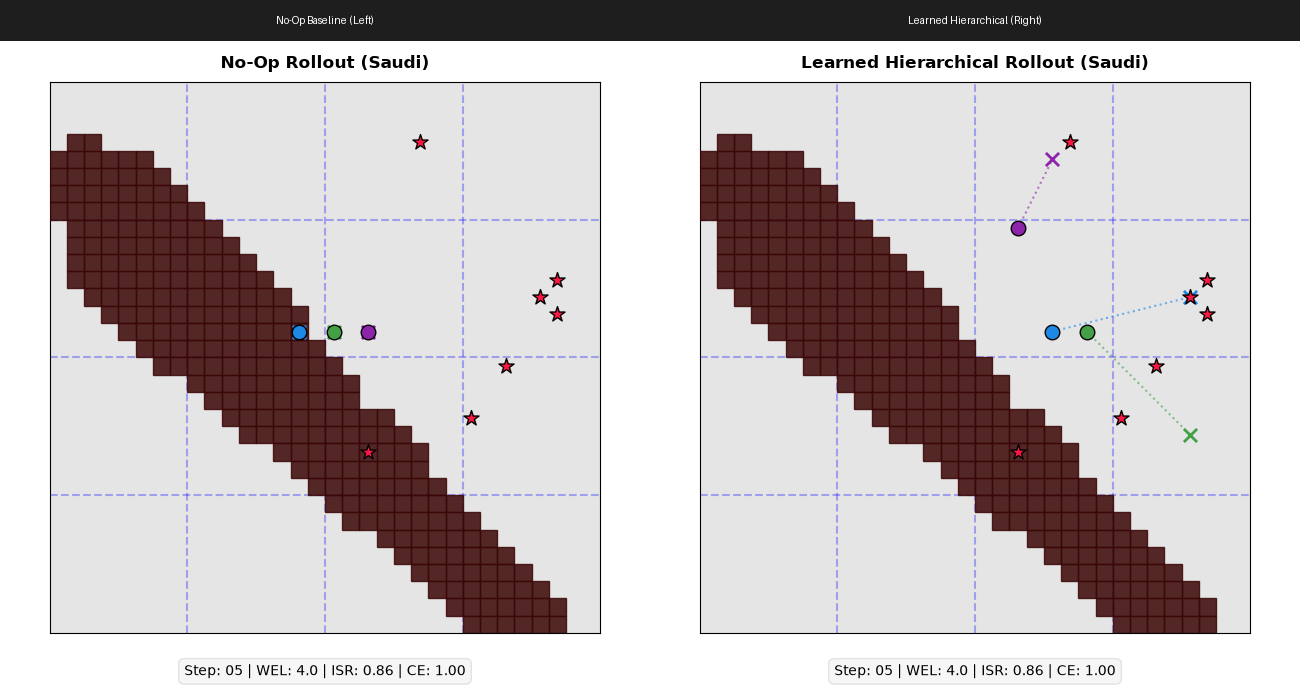
\includegraphics[width=\columnwidth]{Figures/comparison_flat_vs_hier.png}
    \caption{\textbf{Qualitative rollout comparison} (Saudi, seed 2042, mid-episode snapshot at step 120). \emph{Left:} the retrained Flat MARL policy (MAPPO, 100k steps, trained on the same WEL/ISR objective) clusters its agents (circles) near the interior fire and treats cells (blue) away from the gold infrastructure markers, which all burn (WEL $27.0$, ISR $0.29$). \emph{Right:} the hierarchy positions agents adjacent to high-value assets, keeping several unburned (WEL $15.0$, ISR $0.43$). WEL accumulates as assets burn, so the mid-episode value is below the episode total; the two panels differ in both agent placement and outcome.}
    \label{fig:comparison}
\end{figure}

% --- Figure: Flat MARL failure analysis (behavioral evidence) ---
\begin{figure}[t]
    \centering
    \includegraphics[width=\columnwidth]{Figures/flat_failure_analysis.png}
    \caption{\textbf{Where agents spend time (Saudi).} \emph{Left, center:} time-integrated cell occupancy over all evaluation episodes for Flat MARL and the hierarchy (cyan stars = infrastructure). Flat MARL disperses through the interior; the hierarchy concentrates occupancy on the asset cluster. \emph{Right:} mean Chebyshev distance to the nearest asset per policy---the strategic and communication policies operate $\approx 3\times$ closer to infrastructure than Flat MARL, QMIX, or inaction.}
    \label{fig:failure}
\end{figure}

\paragraph{Finding 2: The hierarchy is comparable to---but not statistically equivalent to---its expert teacher.}
The learned hierarchy tracks its Value-First teacher closely: Saudi WEL $20.28$ vs.\ $19.48$ (Welch $t=-1.77$, $df=8.0$, $p=0.115$), California $24.53$ vs.\ $24.61$ ($t=0.06$, $df=8.0$, $p=0.95$). We deliberately avoid inferring equivalence from non-significance: a TOST at the pre-registered $\pm5\%$ margin \emph{fails} to establish equivalence in either region ($p_{\text{TOST}}=0.36$ Saudi, $0.20$ California), and on Saudi the teacher retains a nominal edge ($d=1.12$). The honest reading is that the hierarchy is a competitive reference solution that neither beats nor is proven equal to the heuristic it clones---consistent with our positioning of it as an interpretable baseline rather than a performance contribution.

\paragraph{Finding 3: No method dominates; the benchmark is diagnostic.}
Ranking reverses across regions (Table~\ref{tab:main_results}): CommNet is best on Saudi ($11.43$; vs.\ hierarchy $t=-5.89$, $df=4.4$, $p=0.003$, $d=-3.72$), whereas a trivial reactive-coverage policy is best on California ($15.13$; vs.\ hierarchy $t=-3.30$, $df=6.9$, $p=0.013$, $d=-2.09$). Concentrated petroleum assets reward learned communication and strategic dispatch; scattered WUI assets reward broad coverage. This reversal is the benchmark's central diagnostic property: it discriminates between coordination strategies that a single-region evaluation would conflate, and it is why we present the environment and this comparison, rather than any one controller, as the contribution.

% ====================================================================
% 7. COMPLIANCE AND INTERPRETABILITY ANALYSIS
% ====================================================================
\section{Compliance and Interpretability}
\label{sec:compliance}

The decoupled architecture closes the compliance gap \emph{by construction}: because the tactical layer deterministically seeks the assigned sector, the commander's decisions necessarily control spatial allocation. We therefore do not present compliance as a discovered result; instead we \emph{verify} the guarantee holds in implementation and quantify the resulting behavior with three diagnostics (Table~\ref{tab:compliance}), archived over the full 5-seed protocol.

\begin{table}[t]
\centering
\caption{\textbf{Tactical compliance diagnostics} (5 seeds $\times$ 15 episodes; mean\,$\pm$\,SD). Compliance is $1.000$ by construction; drift and latency are behavioral consequences.}
\label{tab:compliance}
\vspace{0.5em}
\begin{tabular}{lcc}
\toprule
Metric & Saudi & California \\
\midrule
Target Compliance Rate & $1.000 \pm 0.000$ & $1.000 \pm 0.000$ \\
Mean Sector Drift (cells) & $1.99 \pm 0.35$ & $2.47 \pm 1.06$ \\
Dispatch Latency (steps) & $0.98 \pm 0.29$ & $1.21 \pm 0.62$ \\
Cross-sector dispatch rate & $27.1\%$ & $36.6\%$ \\
\bottomrule
\end{tabular}
\end{table}

% --- Figure 3: Commander Strategic Overlay ---
\begin{figure}[t]
    \centering
    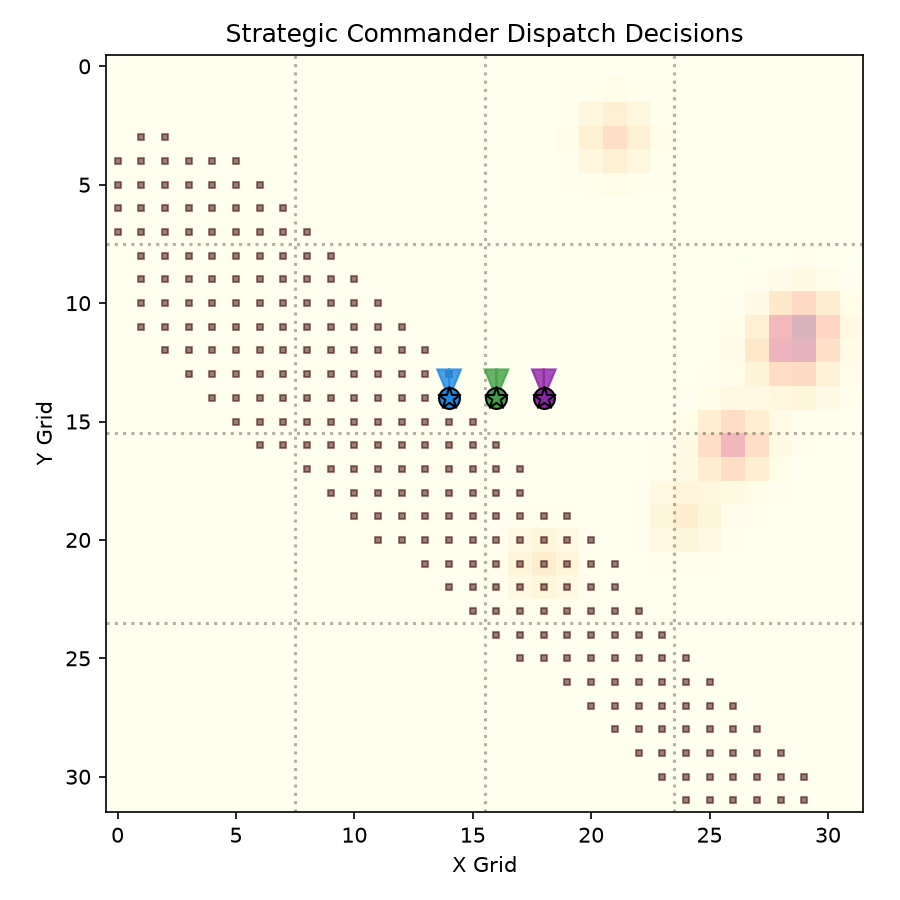
\includegraphics[width=\columnwidth]{Figures/commander_decisions.png}
    \caption{\textbf{Commander dispatch visualization} (Saudi, seed 42, a macro-step with a cross-sector dispatch). Arrows show agent routing from current positions (white circles) to assigned sector centers (blue stars); the $4\times4$ sector grid is overlaid on the fire/asset map (gold stars = infrastructure). Here two of three agents are dispatched \emph{across} sector boundaries toward asset-adjacent sectors. Averaged over all evaluation episodes, the commander dispatches an agent to a sector other than its current one in $27.1\%$ (Saudi) / $36.6\%$ (California) of dispatch events; strategic dispatch is thus a mix of initial placement and periodic cross-sector reallocation, not continuous re-routing.}
    \label{fig:commander}
\end{figure}

\paragraph{Compliance and latency.}
Compliance is $1.000$ in every episode---the intended guarantee, verified free of implementation error. Agents reach within one cell of their assigned sector center in $\approx1$ step on average ($0.98$ Saudi, $1.21$ California), far inside the $T_{\text{macro}}=10$ interval, so they are in position for the bulk of each macro-period.

\paragraph{Reassignment---an honest account of ``strategic dispatch.''}
Mean drift from sector centers is $1.99$/$2.47$ cells, well within the $8\times8$ sectors. Importantly, the commander re-routes an agent \emph{across} sectors in only $27.1\%$ (Saudi) / $36.6\%$ (California) of dispatch events (Figure~\ref{fig:commander}); the remainder keep an agent in its current sector. Strategic behavior is therefore dominated by initial placement plus occasional reallocation, not continuous re-tasking---a caveat that tempers any interpretation of the commander as performing fine-grained dynamic control.

% ====================================================================
% 8. ABLATION ANALYSIS
% ====================================================================
\section{Ablation Analysis}
\label{sec:ablation}

We ablate each design component under the same 5-seed protocol as the main results; the full-system row is \emph{the same runs} as the hierarchy in Table~\ref{tab:main_results} (Table~\ref{tab:ablation}).

\begin{table}[t]
\centering
\caption{\textbf{Component ablation on Saudi Arabia} (5 seeds $\times$ 15 episodes; brackets are 95\% CIs). The full-system row reuses the Table~\ref{tab:main_results} hierarchy runs. $p$ is Welch's test vs.\ the full system.}
\label{tab:ablation}
\vspace{0.5em}
\begin{tabular}{lccc}
\toprule
Configuration & WEL $\downarrow$ & ISR $\uparrow$ & $p$ vs.\ full \\
\midrule
Full System & 20.28 \small{[19.8, 20.9]} & 0.366 & --- \\
BC-only (no RL) & 20.28 \small{[19.6, 20.9]} & 0.366 & $1.00$ \\
\midrule
w/o BC Pretraining & 27.00 \small{[27.0, 27.0]} & 0.286 & $3.0\!\times\!10^{-5}$ \\
w/o KL Regularization & 20.76 \small{[20.3, 21.2]} & 0.360 & $0.31$ \\
w/o Entropy Bonus & 20.76 \small{[20.3, 21.2]} & 0.360 & $0.31$ \\
w/o WEL/ISR Reward & 20.60 \small{[19.6, 21.6]} & 0.362 & $0.64$ \\
w/o Target-Seeking & 27.00 \small{[27.0, 27.0]} & 0.286 & $3.0\!\times\!10^{-5}$ \\
\bottomrule
\end{tabular}
\end{table}

\paragraph{Two components carry the system.}
Removing BC pretraining collapses the commander to No-Op level (WEL $27.00$): pure policy-gradient exploration under sparse, delayed infrastructure reward learns nothing. Replacing the deterministic tactical layer with the (fairly trained, $100$k-step) MAPPO actor \emph{also} collapses the system to $27.00$: the learned actor ignores commander directives, confirming the compliance gap is a real systems issue, not a theoretical one. Both effects are large and significant ($p=3.0\times10^{-5}$).

\paragraph{RL fine-tuning contributes nothing measurable.}
The most informative row is BC-only: removing RL fine-tuning entirely leaves performance unchanged (WEL $20.28$ vs.\ $20.28$; $p=1.00$; TOST-equivalent at $\pm5\%$, $p=0.044$). Consistent with this, the KL, entropy, and reward-shaping ablations move WEL by $<0.5$ and are not significant ($p\geq0.31$). Inspecting weights confirms the mechanism: over $120$ fine-tuning episodes the commander moves $\leq5\times10^{-3}$ from the BC solution and changes none of $200$ probe dispatch decisions. \emph{The learned system is, in effect, behavior cloning of the Value-First heuristic}; the KL-regularized RL stage as configured is inert. We report this plainly---it is why we frame the hierarchy as a reference solution and identifies improving the fine-tuning stage as clear future work. (Identical rows among the KL/entropy/reward ablations follow from this inertness combined with WEL taking discrete values on a coarse lattice.)

% ====================================================================
% 9. TRANSFER ANALYSIS
% ====================================================================
\section{Generalization Analysis}
\label{sec:transfer}

% --- Figure 4: Held-out generalization (replaces the retired TRS heatmap) ---
\begin{figure*}[t]
    \centering
    \includegraphics[width=0.92\textwidth]{Figures/generalization.png}
    \caption{\textbf{Held-out generalization}, measured as $\Delta$WEL $=$ WEL(No-Op) $-$ WEL(policy) computed \emph{within} each condition, so No-Op scores $0$ by construction and a policy that fails to help is visibly on the zero line. Under held-out ignitions and shifted wind, the strategic and communication policies retain value; under a rotated asset layout and cross-region transfer, the hierarchy and its heuristic teacher collapse to the No-Op line while the egocentric policies (Local Reactive, CommNet) still adapt.}
    \label{fig:transfer}
\end{figure*}

We measure generalization by re-evaluating trained policies under four held-out conditions---novel ignition cells, wind rotated $90^\circ$, a rotated infrastructure layout, and cross-region deployment---and scoring each as its WEL improvement over a No-Op baseline \emph{run in the same condition} (Figure~\ref{fig:transfer}). Unlike a reward-ratio transfer score, this metric is falsifiable: No-Op scores exactly $0$, so a policy that adds no value is indistinguishable from inaction. Two findings follow. First, generalization is \emph{structure-dependent}: under held-out ignitions and shifted wind the strategic and communication policies retain most of their value (e.g.\ Saudi CommNet $\Delta$WEL $+17.6$ and $+24.6$ respectively), but under a rotated asset layout the sector-dispatch policies---the learned hierarchy and its Value-First teacher---fall to the No-Op line ($\Delta$WEL $+0.0$/$+0.08$ Saudi), while the egocentric Local Reactive and CommNet policies still adapt. Second, \emph{cross-region transfer is essentially absent}: a policy trained on one region and deployed on the other improves on No-Op by at most $\Delta$WEL $+0.43$ in either direction. The commander's learned sector preferences do not transfer to novel infrastructure geometries.

% ====================================================================
% 10. LIMITATIONS
% ====================================================================
\section{Limitations}
\label{sec:limitations}

We acknowledge several limitations:

\paragraph{The hierarchy's RL stage is inert.}
As Section~\ref{sec:ablation} shows, our KL-regularized fine-tuning does not measurably improve on behavior cloning; the learned commander is effectively a clone of the Value-First heuristic. Making the RL stage productive---e.g.\ a weaker KL anchor, a stronger baseline, or a learned tactical layer---is the clearest path to a hierarchy that \emph{beats} rather than matches its teacher.

\paragraph{Reward--metric coupling and evaluation scope.}
The commander's training reward is a function of the same WEL/ISR quantities used for evaluation; while the baselines share this objective (removing relative confound), absolute performance should be read with that coupling in mind. All results use a single simulator (Cell2Fire), a single month of weather, and asset-criticality rasters that are stylized rather than economically measured (Appendix~G); cross-simulator and multi-season validation remain open.

\paragraph{Scale and generalization boundaries.}
We evaluate $N\in\{3,6,10\}$ agents on $32\times32$ grids. The learned hierarchy is architecturally fixed to $N=3$ (per-agent commander heads) and does not scale without redesign; the communication and reactive baselines do scale (Section~\ref{sec:transfer}). Larger grids ($64^2+$) require rebuilding the infrastructure rasters and retraining and are left to future work. Finally, generalization is limited: the hierarchy's learned sector preferences collapse to No-Op level under rotated layouts and do not transfer across regions (Figure~\ref{fig:transfer}).

\paragraph{Fire dynamics.}
Each agent step advances the simulator one simulated hour and the fire evolves every step; nonetheless the episode horizon ($\sim150$ hours) captures a single fire's active phase rather than a multi-day campaign.

% ====================================================================
% 11. BROADER IMPACTS
% ====================================================================
\section{Broader Impacts}
\label{sec:impacts}

Wildfire suppression research has clear positive potential: effective coordination can save lives and protect critical infrastructure. However, we emphasize that our system operates on a \emph{simulated} environment and is not validated for real-world deployment. Autonomous wildfire suppression decisions could lead to negative outcomes if deployed without human oversight, particularly in scenarios involving civilian evacuation or resource triage. We advocate for AI-assisted decision support rather than fully autonomous suppression.

% ====================================================================
% 12. CONCLUSION
% ====================================================================
\section{Conclusion}
\label{sec:conclusion}

We presented an infrastructure-aware wildfire-coordination benchmark on validated Cell2Fire physics with documented GIS landscapes, and used it to diagnose how decentralized, communication-based, hierarchical, and heuristic controllers behave under a uniform, reproducible protocol. The benchmark is discriminating: policy classes reverse rank across regions, so no single method dominates. It isolates a concrete failure---communication-free MAPPO cannot defend concentrated infrastructure even with a fair budget, while a learned communication channel repairs it---locating the bottleneck in inter-agent coordination. Our behavior-cloned hierarchical commander serves as an interpretable reference solution with compliance guaranteed by construction; we report honestly that its RL stage does not improve on cloning, that it is comparable to but not equivalent to its teacher, and that its learned preferences do not transfer to unseen layouts. We release the code, checkpoints, GIS pipeline, and hashed manifests, and hope the benchmark supports future work on when---and by what mechanism---coordination can be learned for spatially critical suppression.

% ====================================================================
% REFERENCES
% ====================================================================
% \bibliographystyle is issued by aaai2027.sty itself; a second call here would
% produce a duplicate \bibstyle in the .aux and a BibTeX error.
\bibliography{aaai2027}

% ====================================================================
% APPENDIX
% ====================================================================
\onecolumn
\appendix
\section*{Appendix}

\subsection*{A. Hyperparameters}

\begin{table}[h]
\centering
\caption{Training and architecture hyperparameters.}
\label{tab:hyperparams}
\begin{tabular}{ll}
\toprule
Parameter & Value \\
\midrule
\multicolumn{2}{c}{\textbf{Environment}} \\
Grid size & $32 \times 32$ \\
Number of agents & 3 \\
Crop size (egocentric observation) & $9 \times 9$ \\
Max episode steps & 150 \\
Simulated minutes per agent step & 60 (fire advances every step) \\
Coordination penalty & 0.1 \\
Infrastructure catastrophe weight & 2.0 \\
Wrapper cascade probability & 0.1 \\
\midrule
\multicolumn{2}{c}{\textbf{Strategic Commander}} \\
Number of sectors ($M$) & 16 ($4 \times 4$) \\
Macro-step interval ($T_{\text{macro}}$) & 10 \\
Commander MLP hidden dim & 128 \\
Commander (RL) learning rate & $5 \times 10^{-5}$ \\
\midrule
\multicolumn{2}{c}{\textbf{BC Pretraining}} \\
BC episodes & 40 \\
BC learning rate & $1 \times 10^{-3}$ \\
BC epochs & 100 \\
\midrule
\multicolumn{2}{c}{\textbf{RL Fine-Tuning}} \\
RL episodes & 120 \\
KL penalty coefficient ($\lambda$) & 0.3 \\
Entropy bonus coefficient ($\beta$) & 0.05 \\
EMA baseline smoothing ($\alpha$) & 0.1 \\
Reward ISR weight ($\alpha_{\text{ISR}}$) & 20 \\
Optimizer & Adam \\
\midrule
\multicolumn{2}{c}{\textbf{Decentralized baselines (MAPPO / QMIX / CommNet)}} \\
Training environment steps & 100,000 \\
Training objective & WEL/ISR (Eq.~\ref{eq:reward}) \\
Actor / agent CNN features & 64 \\
Critic / mixer hidden dim & 128 \\
MAPPO GAE $\lambda$ / PPO clip & 0.95 / 0.2 \\
QMIX target update interval & 200 \\
CommNet communication rounds & 2 \\
\bottomrule
\end{tabular}
\end{table}

All hyperparameter values above are extracted from the released checkpoint configurations; the training seed is $42$ throughout, and evaluation uses seeds $\{42, 1042, 2042, 3042, 4042\}$ (15 episodes each). Compute and software versions are disclosed in Appendix~F.

\begin{figure}[h]
    \centering
    \includegraphics[width=\columnwidth]{Figures/baseline_training_curves.png}
    \caption{\textbf{Decentralized-baseline training curves} (rolling mean over 25 episodes, $100$k environment steps on the WEL/ISR objective). Convergence evidence for the baseline validity: on Saudi, Flat MARL (MAPPO) plateaus at the No-Op WEL level despite the full budget, whereas CommNet learns to defend infrastructure; on California, MAPPO improves while QMIX does not. This distinguishes genuine coordination failure from an undertrained baseline.}
    \label{fig:curves}
\end{figure}

\subsection*{B. Per-Seed Results}

\begin{table}[h]
\centering
\caption{Per-seed WEL (seeds $42,1042,2042,3042,4042$) for the hierarchy and its Value-First teacher; the seed mean is the unit of analysis.}
\label{tab:per_seed}
\begin{tabular}{lccccc}
\toprule
Policy, Region & S1 & S2 & S3 & S4 & S5 \\
\midrule
Hierarchical, Saudi & 20.6 & 19.8 & 21.4 & 19.8 & 19.8 \\
Value-First, Saudi & 19.0 & 19.0 & 20.6 & 19.0 & 19.8 \\
Hierarchical, California & 24.2 & 26.5 & 26.5 & 22.0 & 23.4 \\
Value-First, California & 24.2 & 26.9 & 26.5 & 22.0 & 23.4 \\
\bottomrule
\end{tabular}
\end{table}

\subsection*{C. Statistical Test Details}

Welch's $t$-tests on seed means ($n=5$), with Welch--Satterthwaite $df$; Cohen's $d$ pooled-SD (sign: policy $-$ reference on WEL, so negative $d$ = policy has lower WEL).

\begin{table}[h]
\centering
\caption{Key WEL comparisons under the uniform protocol.}
\label{tab:statistics}
\begin{tabular}{llccc}
\toprule
Region & Comparison & $t$ ($df$) & $p$ & $d$ \\
\midrule
\multirow{3}{*}{Saudi}
& Hier vs.\ Value-First & $-1.77$ (8.0) & 0.115 & $-1.12$ \\
& Hier vs.\ Flat MARL & $21.0$ (4.0) & $3.0\!\times\!10^{-5}$ & $13.28$$^{\dagger}$ \\
& CommNet vs.\ Hier & $-5.89$ (4.4) & 0.003 & $-3.72$ \\
\midrule
\multirow{3}{*}{California}
& Hier vs.\ Value-First & $0.06$ (8.0) & 0.952 & $0.04$ \\
& Hier vs.\ Flat MARL & $-0.85$ (7.7) & 0.420 & $-0.54$ \\
& CommNet vs.\ Hier & $-3.30$ (6.9) & 0.013 & $-2.09$ \\
\bottomrule
\end{tabular}
\end{table}

\noindent$^{\dagger}$The Flat MARL / No-Op WEL distribution is degenerate (zero variance at $27.0$), so this large $d$ reflects a near-constant comparator and should be read as ``clearly separated,'' not as a calibrated effect size.

\paragraph{Equivalence (TOST).} With a pre-registered $\pm5\%$-of-reference margin, the hierarchy is \emph{not} equivalent to Value-First (Saudi $p_{\text{TOST}}=0.36$; California $0.20$), whereas the BC-only commander \emph{is} equivalent to the full system (Saudi $p_{\text{TOST}}=0.044$)---i.e.\ RL fine-tuning adds nothing detectable.

\subsection*{D. Checkpoint Hashes}

\begin{table}[h]
\centering
\caption{SHA-256 hashes (first 16 characters) of the released checkpoints for every learned policy reported in this paper. Non-learned policies (No-Op, Value-First, Greedy-Risk, Local Reactive) carry no checkpoint.}
\label{tab:hashes}
\begin{tabular}{ll}
\toprule
Checkpoint & SHA-256 (first 16 characters) \\
\midrule
\texttt{checkpoint\_hierarchical\_saudi.pt} & \texttt{43a437aff0ee402e} \\
\texttt{checkpoint\_hierarchical\_california.pt} & \texttt{d7c918dbff61b450} \\
\texttt{checkpoint\_mappo\_saudi.pt} & \texttt{4224a6c690208258} \\
\texttt{checkpoint\_mappo\_california.pt} & \texttt{3ac706e5912eb6a1} \\
\texttt{checkpoint\_qmix\_saudi.pt} & \texttt{c9232eab437b2837} \\
\texttt{checkpoint\_qmix\_california.pt} & \texttt{5af79f6fcfaf53d8} \\
\texttt{checkpoint\_commnet\_saudi.pt} & \texttt{33e76fee0703d216} \\
\texttt{checkpoint\_commnet\_california.pt} & \texttt{b17b36882a52b81e} \\
\bottomrule
\end{tabular}
\end{table}

\subsection*{E. Simulator: Cell2Fire Physics vs.\ Wrapper}

To avoid overstating what is physically validated, we delineate exactly which components come from Cell2Fire and which are our custom wrapper.

\paragraph{Cell2Fire (validated physics).} The fire spread itself is computed by the Cell2Fire C++ engine \citep{pais2021cell2fire}, which implements the Canadian Forest Fire Behavior Prediction (FBP) System: FBP fuel types (mapped from remote-sensing NDVI; Appendix~G), wind- and slope-driven directional rate of spread, one fire period $=1$ simulated minute, and stochastic spread governed by the rate-of-spread coefficient of variation. We invoke it through an interactive stdin/stdout step protocol.

\paragraph{Custom wrapper (not part of Cell2Fire/FBP).} The following are our additions and should not be read as validated fire physics: (i) the \emph{suppression/treatment} action model; (ii) the infrastructure \emph{cascade} model (per-neighbor ignition probability $0.1$ when an asset cell burns) --- the ``cascade probability'' of Appendix~A is a wrapper parameter, not an FBP concept; (iii) the infrastructure-weighted reward (Eq.~\ref{eq:reward}); (iv) the PettingZoo \texttt{ParallelEnv} multi-agent layer with action masking (agents cannot move off-grid or treat non-fuel cells). Each agent step advances the simulator by $60$ fire periods (one simulated hour), so the fire evolves at every step.

\subsection*{F. Compute and Reproducibility Disclosure}

All experiments in this paper ran on a single workstation, CPU-only (no GPU/CUDA was used):
\begin{itemize}
    \item \textbf{Hardware:} AMD Ryzen 5 5600H (6 cores / 12 threads), $\approx 7$\,GB RAM.
    \item \textbf{Software:} Linux (WSL2, kernel 6.6); Python 3.12.3; PyTorch 2.12.1, NumPy 1.26.4, Gymnasium 1.0.0, PettingZoo 1.26.1, SciPy 1.17.1, pandas 2.3.3, Matplotlib 3.11.0.
    \item \textbf{Wall-clock:} each decentralized baseline trains for $100$k environment steps in $\approx 1.7$\,h (California) to $2.5$\,h (Saudi); a full 5-seed $\times$ 15-episode evaluation of all policies takes $\approx 1.5$\,h per region.
    \item \textbf{Seeds:} training seed $42$; evaluation seeds $\{42, 1042, 2042, 3042, 4042\}$ with disjoint train/eval streams. All reported means are over the five evaluation-seed means ($n=5$).
\end{itemize}
A release manifest binds every checkpoint and result artifact to its SHA-256 hash.

\subsection*{G. Data Provenance}

The two regions are built from public remote-sensing sources over a June 2025 window; raw data is not redistributed but is downloaded from the providers and processed deterministically into $32\times32$ Cell2Fire landscapes (converter \texttt{wildfire\_marl.data.to\_cell2fire}; every landscape carries a \texttt{conversion\_report.json} binding it to its input hashes).

\begin{itemize}
    \item \textbf{Regions / ROIs:} Saudi Eastern Province (lon/lat $[45.5, 23.5, 50.5, 28.5]$, desert regime) and Northern California (lon/lat $[-124.5, 36.5, -119.0, 41.5]$, forest/mountain). CRS EPSG:4326, north-up.
    \item \textbf{Fuels:} MODIS NDVI $\rightarrow$ Canadian FBP fuel classes via fixed, region-independent thresholds (Forestry Canada Fire Danger Group 1992; \citealp{pais2021cell2fire}). A declared sensitivity parameter.
    \item \textbf{Weather:} ERA5 (Copernicus) June-2025 extracts $\rightarrow$ hourly \texttt{Weather.csv}; FWI codes via the standard CFFDRS equations. Wind direction is the meteorological from-direction.
    \item \textbf{Topography:} SRTM DEM (public domain) $\rightarrow$ per-cell slope percent and uphill azimuth in FBP convention.
    \item \textbf{Ignitions:} NASA FIRMS detections restricted to burnable cells, detection-count-weighted with disjoint train/eval seed streams.
    \item \textbf{Infrastructure criticality.} The asset-criticality raster is a \emph{stylized} layer (Gaussian value falloff around public infrastructure locations), not measured economic valuations; it is a declared modeling choice, and asset values are a sensitivity parameter rather than ground truth.
    \item \textbf{Resolution abstraction.} \texttt{Forest.asc} declares Cell2Fire's validated 100\,m operating cell size while spatial patterns derive from coarser ROI tiles; absolute geographic distance is not preserved.
    \item \textbf{Known data debt.} The raw California NDVI GeoTIFF was not archived, so California NDVI is reconstructed under a declared linear assumption; this is covered by the fuel-map sensitivity analysis and flagged for closure by re-download.
    \item \textbf{Release.} Code, configs, checkpoints (Appendix~D), and the generated landscapes are released with a SHA-256 manifest; a fixed snapshot may be archived on Zenodo with a DOI.
\end{itemize}

\end{document}
